\section{Simulations et tests d'intégration}
Cette section détaille les tests à réaliser lors de l'intégration.
Une sous-partie présente également pourquoi une simulation ne semble pas apporter tout son potentiel dans le contexte du projet.
Plusieurs mentions sont faites à l'automatisation des tests par la suite.
Nous sous-entendons par cela la nécessité d'écrire un programme appliquant une entrée choisie et comparant le résultat avec la valeur attendue.
Cette méthode s'oppose à la validation manuelle visant à observer la conformité des chronogrammes un à un.
Nous défendons l'idée d'automatiser les tests et d'utiliser les chronogrammes pour le debug uniquement.
Au début, un temps plus important doit être investi à l'écriture des programmes de test.
Il est très probable que des problèmes soient découverts lors des tests et que certaines étapes doivent être répétées plusieurs fois.
In fine, il semble y avoir un gain de temps évident à l'automatisation en plus d'une meilleure traçabilité et répétabilité.


\subsection{Les tests d'intégration}

Il s'agit dans la sous-section suivante de présenter les différents tests d'intégrations.
Les points ci-dessous présentent les divers tests avec une brève présentation, les éléments validant la bonne intégration de l'IP.
Pour chacune de ces étapes, les outils Xilinx Vivado et Xilinx SDK seront employés.
L'ordre des tests importe car ils sont dépendants, le dernier ne pourra être conforme sans la validité du premier.
% ajout de subsubsection* ou numéro liste

\subsubsection*{Écriture et lecture}

Le CPU effectue des cycles d'écriture et de lecture pour chaque registre de l'IP.
La valeur écrite doit toujours être identique à celle lue un instant plus tard.
Il peut être particulièrement intéressant d'effectuer une écriture dans tous les registres avec des valeurs différentes connues puis une lecture pour vérification.
Il est ainsi possible de détecter les problèmes d'écriture dans deux registres à la fois.
En cas de non conformité ou pour s'assurer que le test s'exécute correctement, un ILA est placé sur l'interface AXI4-Lite et permet d'observer les signaux (VALID,READY) et les bus (ADDR,DATA) de chaque canal (canal d'écriture et canal de lecture).

\subsubsection*{Fonctionnement global lors d'une seule interruption}

Les lignes d'interruptions de chaque bloc sont testées une à une.
Une interruption peut être générée lors d'un usage normal d'une IP, mais cela complexifie énormément le test du contrôleur d'interruptions.
Pour palier à cela, la génération des signaux d'interruption peut normalement se faire par écriture dans le registre d'ISR.
Chaque signal d'interruption à l'état bas devra générer un chargement d'une nouvelle adresse de branchement et le passage à zéro de \texttt{IT\_CPU}.
L'adresse de branchement devra être configurée au préalable et comparée à la valeur lue.
Cette étape semble facilement automatisable à l'aide d'un code C et pourra être réutilisé dans le test de couverture plus bas.
De nouveau, en cas de problème ou pour s'assurer de la conformité du test, un bloc ILA peut être instancié et connecté aux lignes d'interruptions de chaque IP et la ligne d'interruption \texttt{nIT\_CPU}.
Les breakpoints de Xilinx SDK seront utiles pour approfondir l'inspection si besoin.

\subsubsection*{Fonctionnement global lors de multiples interruptions}

Pour finir, des tests simultanés doivent être effectués avec les IT des diverses IP sous plusieurs configurations (niveau de priorité différent, masquage ou non etc).
Les éléments de validation sont les mêmes que le point précédent à quoi on ajoute la conformité dans l'ordre d'exécution.
Ce cas un peu plus complexe que le premier semble tout à fait automatisable via du logiciel.
L'exemple suivant éclairera ce propos. 

%\begin{itemize}
%	\item Le CPU effectue des cycles d'écriture et de lecture pour chaque registre de l'IP.
%	La valeur écrite doit toujours être identique à celle lue un instant plus tart.
%	Il peut être particulièrement intéressant d'effectuer une écriture dans tous les registres avec des valeurs différentes connues puis une lecture pour vérification.
%	Il est ainsi possible de détecter les problèmes d'écriture dans deux registres à la fois.
%	En cas de non conformité ou pour s'assurer que le test s'exécute correctement, un ILA est placé sur l'interface AXI4-Lite et permet d'observer les signaux (VALID,READY) et les bus (ADDR,DATA) de chaque canal (canal d'écriture et canal de lecture).
%	 couplage indirecte ?? Pas vraiment besoin de dma lorsque les registres sont unitaires 
%	\item Dans une cas de couplage indirect, l'IP doit également coopérer avec le DMA afin de transférer des données de l'IP vers les mémoires vives.
%	Les éléments de validation sont les mêmes que le point précédent.
%	\item Les lignes d'interruptions de chaque bloc sont testées une à une.
%	Une interruption peut être générée lors d'un usage normal d'une IP, mais cela complexifie énormément le test du contrôleur d'interruption.
%	Pour palier à cela, la génération des signaux d'interruption peu normalement se fait par écriture dans le registre d'ISR.
%	Chaque signal d'interruption à l'état bas devra générer un chargement d'une nouvelle adresse de branchement et le passe à zéro de \texttt{IT\_CPU}.
%	L'adresse de branchement devra être configurée au préalable et comparée à la valeur lue.
%	Cette étape semble facilement automatisable à l'aide d'un code C pourra être réutilisé dans le test de couverture plus bas.
%	De nouveau, en cas de problème ou pour s'assurer de la conformité du test, un bloc ILA peut être instancié et connecté aux lignes d'interruptions de chaque IP et la ligne d'interruption \texttt{nIT\_CPU}.
%	Les breakpoints de Xilinx SDK seront utiles pour approfondir l'inspection si besoin.
%	\item Pour finir, des tests simultanés doivent être effectués avec les IT des diverses IP sous plusieurs configurations (niveau de priorité différent, masquage ou non etc).
%	Les éléments de validation sont les mêmes que le point précédent à quoi on ajoute la conformité dans l'ordre d'exécution.
%	Ce cas un peu plus complexe que le premier semble tout à fait automatisable via du logiciel.
%	L'exemple suivant éclairera ce propos. 
%\end{itemize}

Par exemple, il existe deux configurations possibles (priorité et masquage) pour l'ensemble des 15 interruptions.
Le triplet (IT, priorité, masquage) offre $15\times8\times2$ soit $240$ combinaisons possibles comme le présente la figure ci-dessous.

\begin{figure}[h!]
	\centering
	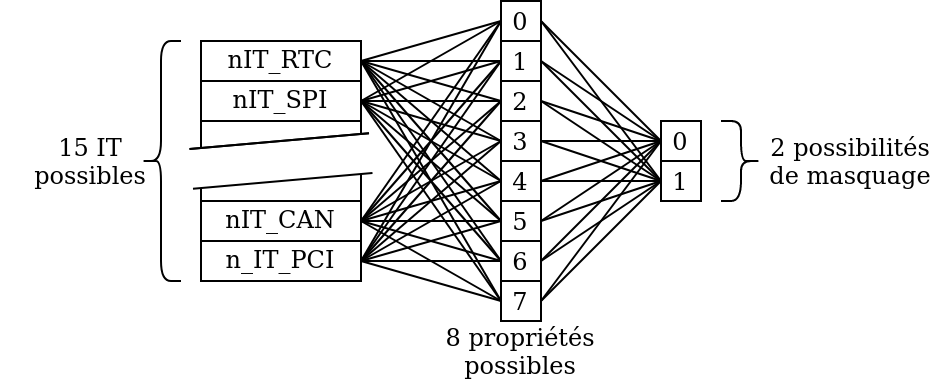
\includegraphics[width=0.7\linewidth]{figure/combinaisons_integration.png}
	\caption{Exemple de couverture de tests d'intégrations}
	\label{fig:combinaisons_integration}
\end{figure}

Il s'agit de couvrir l'ensemble des 240 triplets possibles tout en vérifiant que les priorités des interruptions soient respectées. 
Pour se faire, 14 IT ont une priorité fixe et seulement 1 varie selon le niveau de priorité et le masquage.
La génération du signal d'interruption se fera toujours par écriture dans les registres ISR.
Cela peut être programmé et le résultat inscrit dans un fichier de log.

\subsection{Étapes non nécessaires}

À ce stade du développement de l'IP, certaines étapes étudiées ne sont pas nécessaires.

\subsubsection*{Utilisation de SystemC}

Par exemple, les étapes de modélisation et de vérification au niveau système réalisable sur SystemC.
Il n'y a aucun profit à tirer de cet outil car l'IP est déjà décrite et la spécification et conception au niveau système ont déjà été pensées.

\subsubsection*{Utilisation de Intel CoFluent}

En ce qui concerne l'outil de codesign Intel CoFluent étudié en travaux pratiques, celui-ci est utile en amont de la conception.
CoFluent permet de réaliser des études de faisabilité, déterminer des propriétés pour un circuit donné et effectuer du design exploration.

%\begin{itemize}
%	\item Par exemple, les étapes de modélisation et de vérification au niveau système réalisable sur SystemC.
%	Il n'y a aucun profit à tirer de cet outil car l'IP est déjà décrite et la spécification et conception au niveau système ont déjà été pensées.
%	\item En ce qui concerne l'outil de codesign Cofluent étudié en travaux pratiques, celui-ci est utile en amont de la conception.
%	Cofluent permet de réaliser des études de faisabilité, déterminer des propriétés pour un circuit donné et effectuer du design exploration.
%\end{itemize}


